\RequirePackage[T1]{fontenc}
\documentclass[conference,10pt]{IEEEtran}
\usepackage{amsmath,amssymb,graphicx,url}
\newcommand{\Rone}{\mathrm{R1}}
\newcommand{\Azero}{\mathrm{A0}}
\newcommand{\Btwo}{\mathrm{B2}}
\newcommand{\pct}{\%}
\title{Reachability-Constrained Shared-Crossing Planning for 3D FPGA Routing}
\author{\IEEEauthorblockN{Anonymous submission draft}}
\begin{document}
\maketitle
\begin{abstract}
Vertical connectivity complicates timing-driven FPGA routing because feasible crossings differ across sinks and architectures. We develop a reachability-constrained planner that compares shared and split crossing assignments on a finite terminal hierarchy, then softly guides VTR routing. Controlled experiments separate routing, placement, and toolchain effects across three architectures. On complete dual-baseline cohorts of two to four circuits, timing changes range from a 0.64\% regression to a 1.32\% improvement; larger individual gains coexist with regressions and failures. All ten valid serial timing groups incur overhead. Mechanism analysis exposes sparse delay coverage and motivates a controlled test of the planner's independent contribution.
\end{abstract}
\begin{IEEEkeywords}
3D FPGA, detailed routing, vertical interconnect, dynamic programming, architecture exploration
\end{IEEEkeywords}

\section{Introduction}
Stacking FPGA layers changes the routing decisions that translate architectural resources into performance. A net may share vertical crossings among branches or select separate crossings for critical sinks. Nearby resources may be unreachable through the directed routing resource graph (RRG), and reachable choices may become poor after congestion negotiation or a critical-path change.

Recent tools enable detailed exploration of three-dimensional fabrics. VTR supports 3D architectures, LaZagna generates flexible vertical connectivity, and Escaping Flatland improves the placement flow used to assess these fabrics~\cite{vtr9,vtr9paper,lazagna,flatland}. These advances make it possible to ask a narrower routing question: with the packed netlist, placement, architecture, and timing model fixed, does coordinating crossing choices across a net improve its final routed timing? Answering this question requires distinguishing a routing modification from the benefit of a different placement or a different toolchain.

We investigate a planner that represents legal crossing choices explicitly and compares sharing against splitting within a deterministic hierarchy of remote terminals. The planner combines directed reachability, spatial candidate reduction, criticality filtering, and optional bounded delay queries. Its output is a soft preference used by the existing detailed router. Feasible resources remain available, and the final route is judged by the ordinary routing and timing checks. The implementation is based on a fixed VTR 9 development revision; it is not a new fabric generator or placer.

Our contributions are a finite shared-crossing objective with explicit fallback behavior; fixed-input evaluation across switch-block (SB), output connection-box (CB-O), and hybrid (Hybrid-O) connectivity, separating two placement flows and three baseline identities; and mechanism analysis connecting improvements and regressions to coverage, final resources, changing worst paths, and runtime costs.

The results support conditional timing effects, not a general performance victory. On the complete cohorts used for the paired 3D/2D display, mean routing improvements range from $-0.64\%$ to $1.32\%$, with only two to four circuits contributing to each mean. A single Hybrid-O case improves by $12.96\%$, while another worsens by $11.45\%$. All ten serial groups with three legal paired repetitions are slower than the native baseline. These outcomes make coverage and attribution central to the contribution: a resource-efficient route or a better isolated example does not establish lower critical-path delay across the suite.

\section{Related Work}
VTR provides FPGA architecture and CAD infrastructure~\cite{vtr8}; version 9 added 3D support~\cite{vtr9}. The 3D extensions studied by Boutros et al. connect device models with CAD-level exploration~\cite{third}. We use that infrastructure and retain its detailed router, timing analysis, and legality checks. The new element is a crossing-selection layer above detailed connection search, with a deliberately limited optimization objective.

LaZagna supports architecture generation and evaluation beyond a single vertical-connectivity template~\cite{lazagna}. Its original published VTR 8.1 results and the later VTR 9-code port are different baselines. Neither is interchangeable with the official-source VTR derivative used here. Escaping Flatland addresses partitioning, delay estimation, annealing costs, and moves during placement~\cite{flatland}; our routing comparison instead holds each resulting placement fixed. Its architecture-ranking observations motivate checking rankings, rather than predicting that another routing method must reproduce a reversal.

H3D optimizes bonding-terminal number and positions for face-to-face IC global routing~\cite{h3d}. We borrow the shared-crossing idea, not its geometric model or guarantees. Our finite hierarchy handles directed, prefabricated FPGA resources; it is neither H3D's algorithm nor a global FPGA Steiner-tree solver. Dynamic programming and strongly connected components are established tools, not standalone novelty claims.

\clearpage
\section{Problem Model}
Let $G=(V,E)$ be a directed RRG. Each resource $v$ has capacity $u_v$, physical location and layer, and an associated routing cost. Edges identify actual connections and switches. For each net $n$, source $s_n$ and terminals $T_n$ are fixed by a packed netlist and placement. Detailed routing selects connected legal trees subject to shared capacities, while timing analysis evaluates the resulting circuit. We restrict the planner to two layers and clustered, serial routing.

A crossing candidate $c$ denotes a real vertical entry resource, not a freely placeable via. In the evaluated edge encoding, SB crossings use paired half-nodes and CB-O crossings originate at an output pin. Different CB edges can share the same output resource; counting every edge as an independent via would overstate capacity. A native CHANZ representation is supported separately, but is not silently equated with these edge-encoded resources.

For a remote terminal $i$, candidate $c$ is feasible when a same-layer directed path reaches its entry from $s_n$ and an actual crossing exit can reach $i$ on the destination layer. These conditions certify a single-crossing walk in the full graph. They do not certify a congestion-free route for all nets, a route inside the current search bounding box, or the best possible multi-crossing route. Reverse traversal is an analysis operation only; it never adds edges to the router.

Let $C_i$ be the finite candidate table available to terminal $i$, and let $\alpha_i$ be its routing criticality at initial planning. We use an opening proxy $o(c)$ for source access and prospective resource congestion, and a branch proxy $b_i(c)$ for sink access and criticality. A representative form is
\begin{align}
 o(c)&=d_s(c)+\lambda_o a_c[1+p\max(0,q_c-u_c)],\\
 b_i(c)&=(1+4\alpha_i)d_i(c)+4\alpha_i d_s(c).
\end{align}
Here $a_c$ is accumulated congestion cost, $p$ is the present-cost factor, and $q_c$ includes one prospective unit unless the net already owns the resource. Distances are normalized geometry proxies or supported switch-delay estimates. Partial delay coverage can mix measured opening cost and geometric branch cost.

For hierarchy node $v$, let $L(v)$ contain its terminals. The finite objective is
\begin{equation}
 \begin{aligned}
 S(v)&=\min_{c\in\cap_{i\in L(v)}C_i}\left[o(c)+\sum_{i\in L(v)}b_i(c)\right],\\
 D(v)&=\min\{S(v),D(v_l)+D(v_r)\}.
\end{aligned}
\end{equation}
An unavailable shared choice has infinite cost. At a leaf, only the shared term applies. Opening cost is charged per selected hierarchical group; unrelated groups choosing the same resource do not receive an additional global deduplication credit. Physical same-net sharing is instead represented by the actual route tree. This surrogate omits detailed downstream wire sharing and loading, so lowering it need not lower final circuit delay.

\section{Method}
\subsection{Directed feasibility and candidate reduction}
We query the strongly connected component condensation of same-layer edges, preserving directed reachability. Spatial sampling considers endpoints, interpolated locations, and the net centroid. Feasible candidates are ranked by their proxy costs and diversified across sites; feasible crossings already owned by the net remain eligible. If the spatial sample provides no feasible candidate, the planner scans the crossing table for a usable fallback set. Current occupancy does not by itself exclude a resource, because later congestion negotiation may release it.

The pooled candidates from all eligible terminals form the finite DP table. Each terminal is checked against this pool again, and entries with unavailable measured branch cost are omitted from the surrogate. A candidate introduced by one terminal can serve another. The proposed independent-selection ablation must retain this same table.

\subsection{Finite shared/split planning}
Terminals are recursively divided at the median along the larger spatial extent. At each hierarchy node, the recurrence compares one common crossing with the two child solutions. Induction over the hierarchy proves optimality within these alternatives: each allowed partition either shares at the current node or consists of allowed child partitions. This statement does not cover other hierarchies, excluded candidates, or global capacity coupling. Ties favor a shared group, then deterministic candidate order. Nets with more than 128 eligible remote terminals use independent candidate guidance and increment a fallback counter.

\subsection{Budgeted delay scoring and routing integration}
Delay queries perform bounded exploration and cache endpoint results. The implementation accepts its additive switch-delay proxy only for its supported zero-wire-RC model. A truncated search is not an infeasibility proof. Fully delay-scored terminal choices require enough candidates covered by both forward and reverse searches; otherwise geometric terms remain available. We report query, truncation, cache-hit, and fully scored-terminal counts separately.

The selected configuration uses a static guide: each net is planned once, and the guide is reused on later reroutes. Unpreferred crossing resources receive a nonnegative extra congestion preference, while existing timing-driven search and congestion penalties remain active. A failed guided sink search retries without the guide before ordinary recovery. Static caching bounds repeated planning but may preserve an early decision after congestion or criticality changes. This tradeoff is part of the method, not a claim that all later routing states are optimized.

\clearpage
\section{Experimental Setup}
\subsection{Tools, architectures, and comparison identities}
The native baseline A0 and our router R1 derive from official VTR development commit \texttt{0b912334}; R1 adds the planner and graph-encoding integration. Strict serial builds have separate recorded binary identities. B2 is the modern LaZagna port at VTR commit \texttt{5abd3aca}~\cite{modern}, with archived build and compatibility changes. It has been built and exercised under controlled inputs. Its historical version string is not used to infer equivalence with official VTR 9. The original LaZagna VTR 8.1 paper is B1, an external published reference rather than a matched local routing experiment.

We use derived SB, CB-O, and Hybrid-O architectures with a common planar graph and segment mix. Vertical connections retain their generated directions and switch timing. Import checks compare directed connections, switches, and resource semantics between source and native representations. Matching logical capacity does not imply equal area, power, or vertical-interconnect budgets. The modeled wires have zero R/C while switch delays remain; these are architecture experiments, not calibrated silicon predictions.

For each circuit, the registered sizing rule selects the smallest permitted grid side satisfying at most 80\% occupancy for every logical block class. A common size is used across architectures and placement flows. The matched 2D reference preserves logical capacities with a separate near-square layout. Its planar wire-unit inventory differs from 3D by $-0.18\%$ to $+1.87\%$ across the prepared models. It is an architecture/placement denominator, not a fixed-placement routing control. Main measurements use width 100 and ideal clocks, a maximum of 200 routing iterations, disabled failure prediction, a 1800-second route-process limit and a 3600-second placement limit. A 64-GiB address-space cap applies per solver.

\subsection{Placement, selection, and evaluation separation}
P0 is native placement on the paper-packed netlist. P1 executes the paper placement flow, including weighted TritonPart initialization, and repacks to populate criticality information. Packed-netlist semantics are checked against the census. Every A0/R1/B2 routing contrast within a flow uses private copies of the same packed netlist and placement coordinates, with equivalent graph and timing inputs. A P1/P0 contrast changes placement and setup work and is reported separately.

Six training circuits use seed 11: attention\_layer, bnn, eltwise\_layer, gemm\_layer, softmax, and spmv. Fourteen other circuits use evaluation seeds 21, 23, and 25. These circuits had appeared in historical development experiments; the split is fresh for this selection exercise, not evidence of previously unseen benchmark families. Each of four variants---geometry (G), delay (D), criticality (C), and their combination (D+C)---receives eight registered configurations per architecture. All four retain the shared/split DP. Selection prioritizes legal coverage and then circuit-balanced timing on comparable training cases; selected configurations are frozen before evaluation.

\begin{table}[h]
\centering\caption{Frozen selected configurations. $K$ is the candidate target, $\tau$ the criticality threshold, $B$ the per-query settled-node budget. Delay budget is inactive for C.}
\label{tab:config}
\begin{tabular}{lrrrrrr}\hline
Architecture & Variant & $K$ & $\tau$ & $B$ & $\lambda_o$ & Miss\\\hline
SB & C &16&0.80&8192&4&4\\
CB-O & C &8&0.95&1024&4&4\\
Hybrid-O & D+C &16&0.70&4096&16&2\\\hline
\end{tabular}
\end{table}
The held-out main schedule has 168 circuit/seed/architecture cases, including matched 2D cases, with multiple routing roles per case. The separate transferred-width schedule has 12 cases. Fixed-parameter and equally budgeted selected-parameter ablations use seed 21 and P1. Identical immutable configurations can share one execution through explicit role references; reused executions are not independent observations.

\subsection{Validation, metrics, and aggregation}
A result enters a CPD ratio only after VPR FULL checking and the registered independent directed-edge, switch, tree, and node-capacity audit. The independent checker complements rather than replaces VPR: it does not independently establish every terminal-identity or configuration-closure condition. Failed, timed-out, or unexecuted descendant roles remain in coverage accounting. We never insert zero delay for a missing route.

For circuit $j$, we first average the three seed CPDs within each arm. On a complete paired circuit set $S$, we report
\begin{equation}
 I=100\left[1-\exp\left(\frac{1}{|S|}\sum_{j\in S}\log\frac{\bar d_{j,R1}}{\bar d_{j,base}}\right)\right].
\end{equation}
Positive $I$ denotes improvement. The paired 3D/2D display uses the same complete intersection for both denominators. Legal individual pairs outside that intersection still contribute to the separate win/tie/loss counts. Toolchain comparisons may have a different complete set and cannot be subtracted from these means.

Formal runtime uses three serial repetitions of spmv and robot\_rl, both flows, all architectures, and rotated router order. R1-off controls separate algorithm overhead from build differences. A seccomp guard prevents worker-thread creation without ptrace instrumentation. Registered study processes do not overlap, but the shared host is not exclusive. We report router time, route-process time, and setup costs separately. Parallel-sweep durations are mechanism observations, not speedup evidence.

\clearpage
\section{Results}
\subsection{Timing, failures, and the three baselines}
Table~\ref{tab:main} reports the complete dual-baseline cohorts. Hybrid-O has small positive means in both flows; SB changes sign across flows, and CB-O is unchanged against A0 at reported precision. The 2D comparison can differ substantially because it includes a different physical layout and placement. For example, CB-O/P0 improves by 3.05\% against matched 2D while showing zero routing improvement against its own 3D A0. This is not a routing speed or timing gain attributable to R1.

\begin{table}[h]
\centering\caption{CPD improvement (\%). Parentheses give the matched 2D comparison on the same $n$ complete circuits. Each panel registers 14 circuits and 42 seed samples. W/T/L counts cover all legal R1/A0 seed pairs, not only the complete dual cohort.}
\label{tab:main}
\begin{tabular}{llrrr}\hline
Fabric & Flow & $n$ & vs. 3D (vs. 2D) & W/T/L\\\hline
SB & P0 &3&$-0.64\;(-7.17)$&9/4/10\\
SB & P1 &4&$+0.41\;(+0.89)$&7/6/11\\
CB-O & P0 &2&$0.00\;(+3.05)$&0/11/0\\
CB-O & P1 &2&$0.00\;(+4.28)$&0/12/0\\
Hybrid-O & P0 &3&$+1.32\;(+0.35)$&7/9/7\\
Hybrid-O & P1 &4&$+1.08\;(+1.05)$&11/9/4\\\hline
\end{tabular}
\end{table}

\begin{table}[h]
\centering\caption{Main held-out role outcomes: legal/failed/timeout, 42 roles per cell. Failed includes registered failures and unavailable descendants, not only router nonconvergence.}
\label{tab:coverage}
\begin{tabular}{llrrr}\hline
Fabric&Flow&A0&R1&B2\\\hline
SB&P0&23/11/8&23/10/9&24/10/8\\
SB&P1&24/8/10&24/8/10&24/8/10\\
CB-O&P0&11/27/4&11/27/4&11/27/4\\
CB-O&P1&12/27/3&12/27/3&12/27/3\\
Hybrid-O&P0&24/10/8&23/10/9&24/9/9\\
Hybrid-O&P1&24/12/6&24/11/7&24/12/6\\\hline
\end{tabular}
\end{table}
Failures are substantial, especially for CB-O. The 756 main 3D roles yield 354 legal routes, 280 routing failures, 121 timeouts, and one allocation failure under the registered limit. Matched 2D contributes only 17/42 legal references. Across evaluation including ablations and transferred width, 581/1206 roles are legal, 455 fail, and 170 time out; reuse gives 1136 unique attempts (552/423/161). These are execution counts, not independent circuits. Failed routing logs can contain positive CPDs; such values are excluded.

Against modern LaZagna B2, the R1 mean CPD improvements are $+0.67\%/-1.60\%$ for SB P0/P1, $-0.67\%/+0.57\%$ for CB-O, and $+1.61\%/-2.27\%$ for Hybrid-O. The respective complete-circuit counts are 7/8, 2/2, and 6/8. These are toolchain contrasts on matched inputs. They do not establish that the planner causes every R1/B2 difference, particularly where R1 and A0 tie.

For B1, the original LaZagna paper reports normalized CPDs of 0.821, 0.819, and 0.809 for 100\%, 66\%, and 33\% SB connectivity, respectively, relative to its own 2D reference~\cite{lazagnav1}. Those architectures, circuits, and denominators do not match this experiment. We retain these published values as context and leave the direct R1/B1 ratio undefined. The newer tool port and historical source reproductions do not substitute for the author's published measurement.

The largest same-sample dual gain is Hybrid-O/P0, clstm\_like.small, seed 23: 12.96\% against A0 and 10.54\% against matched 2D. It coexists with an 11.45\% regression for clstm\_like.large, seed 23, in the same architecture and flow. Across SB/P0, robot\_rl seed 21 worsens by 13.30\%. Extremes illustrate sensitivity; none replaces a mean or a failure denominator.

\subsection{Runtime cost and architecture ordering}
All ten R1/A0 groups with three legal serial repetitions incur router overhead, with median ratios from 1.129 to 3.382. The corresponding route-process ratios are 1.047--1.313. Two robot\_rl/CB-O groups lack legal paired repetitions and remain missing rather than neutral. Observed median setup spans 13.59--71.25 s, including 0.84--6.04 s of partition work where applicable. P0 reuses census packing whereas P1 repacks; these are flow-specific costs, not equal-work end-to-end speedups.

The same-build R1-off control also shows overhead in all ten complete groups: R1/R1-off spans 1.180--3.327 for router time and 1.015--1.334 for process time. Against B2, these ranges are 0.906--4.214 and 0.910--1.267; only one and two groups, respectively, are faster. These toolchain differences do not establish overall acceleration.

Only conv\_layer\_hls belongs to the complete intersection across all three architectures and both routing/placement choices. On this circuit's three-seed means, all four combinations rank CB-O, then SB, then Hybrid-O; the strict reversal count is zero. Individual seed rankings change, however: P1 ranks SB first at seed 21 and Hybrid-O first at seed 25, for both A0 and R1. With this limited intersection, neither a general best architecture nor a ranking reversal is supported. Architecture exploration needs robust coverage and a credible physical comparison, in addition to a successful search method.

\begin{figure}[h]
\centering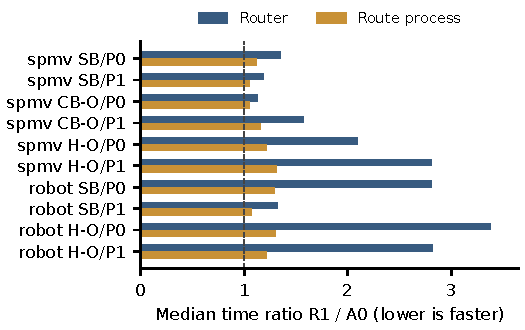
\includegraphics[width=\columnwidth]{figures/strict_runtime.pdf}
\caption{Strict serial timing: all ten complete groups exceed unity. Two registered robot\_rl/CB-O groups have no legal three-repeat pair and are omitted from ratios, not from coverage.}
\label{fig:runtime}
\end{figure}

\clearpage
\section{Mechanism Analysis}
\subsection{Coverage is narrower than the algorithm's name}
The frozen CB-O threshold of 0.95 selects few remote terminals. Across its legal main runs, the mean selected-terminal fraction is 0.142\% for P0 and 0.0143\% for P1; all legal R1/A0 CPDs tie. Sparse guide application is consistent with this lack of a final timing effect, but the counters alone do not establish that a lower threshold would help. A broader guide can also increase work or redirect routing adversely.

Hybrid-O enables delay estimation, yet complete forward/reverse coverage is rare. Its legal P0 runs fully score 32 of 44,064 eligible terminals in aggregate; P1 scores 60 of 43,119. All 32,941 P0 and 46,650 P1 recorded endpoint queries hit their exploration cap. Truncation does not imply an empty query: settled entries remain useful, and measured source costs can affect choices that fall back for branch scoring. The data expose a mismatch between the configured budget and the candidate sets, rather than proving that delay-aware optimization is intrinsically ineffective.

\begin{table}[h]
\centering\caption{Mechanism cases, Hybrid-O/P0, seed 23, W100. Resource values are audited final-route counts; timing costs are observed sweep diagnostics.}
\label{tab:mechanism}
\small\setlength{\tabcolsep}{3pt}
\begin{tabular}{lrr}\hline
Quantity&small CLSTM&large CLSTM\\\hline
CPD A0 $\rightarrow$ R1 (ns)&7.1478 $\to$ 6.2215&7.0737 $\to$ 7.8835\\
SB pairs A0 $\rightarrow$ R1&53 $\rightarrow$ 40&51 $\rightarrow$ 52\\
CB sources A0 $\rightarrow$ R1&1159 $\rightarrow$ 1164&2873 $\rightarrow$ 2870\\
Planar length A0/R1&227162 $\rightarrow$ 227088&629142 $\rightarrow$ 629368\\
Eligible / remote&530 / 3902&1233 / 10863\\
Delay-scored / eligible&2 / 530&2 / 1233\\
Queries / capped&808 / 808&1778 / 1778\\
Planning time (s)&28.73&106.13\\
Router A0 $\rightarrow$ R1 (s)&5.84 $\rightarrow$ 34.78&17.26 $\rightarrow$ 126.24\\
Iterations A0 $\rightarrow$ R1&26 $\rightarrow$ 26&24 $\rightarrow$ 29\\\hline
\end{tabular}
\end{table}

\subsection{An improvement with a different critical path}
For clstm\_like.small, the planner selects 530 of 3902 remote terminals, forms 372 groups, and records no empty-candidate, high-fanout, or guided-search fallback events. The final route uses thirteen fewer SB pairs but five more CB crossing output sources. Planar length falls by only 74 units, or about 0.033\%. The observed CPD gain therefore accompanies a change in route topology rather than a large reduction in total wirelength.

The saved A0 worst path runs through a multiplier in an inverse-transform block. Under R1, the worst path instead lies in an elementwise subtraction block; the start and end registers both change. Its reduced worst delay shows that the overall routing perturbation improves this sample. However, the two saved reports describe different paths, so their component delays cannot be subtracted as if they measured the same connection. In particular, they do not identify which chosen crossing relieved the original worst path. A connection-level causal account would require matched path traces or an additional instrumented control.

Only two eligible terminals receive complete delay scoring. The observed improvement consequently supports the whole selected configuration, not a claim that the bounded delay estimator or DP alone caused it. Planning consumes 28.73 seconds out of 34.78 reported routing seconds, approximately 83\%. The same 26 negotiated-congestion iterations do not imply equal work per iteration. Caching removes repeated planning but does not remove its initial cost.

\subsection{A degradation despite similar resource use}
For clstm\_like.large, CPD increases from 7.07372 to 7.88347 ns. The final route uses one additional SB pair, three fewer CB crossing sources, and 226 more planar-length units, about 0.036\%. These small changes in aggregate resources fail to predict the 11.45\% timing degradation. The worst path changes from one multiplier/register chain to a different inverse-transform multiplier path. The saved reports again support a bottleneck change, not a matched-edge delay decomposition.

The planner forms 938 groups from 1233 eligible terminals, but only two receive complete delay scoring. It records no guided-search, high-fanout, or empty-candidate fallback. Thus fallback activation is not an explanation for this regression. A feasible, cached guide can simply steer congestion negotiation toward a worse final critical path. Planning takes 106.13 of 126.24 router seconds, approximately 84\%, and routing needs 29 iterations instead of 24. This case exposes both proxy mismatch and substantial setup cost.

Pairing final connections by net name, pin index, and identical SOURCE/SINK resource IDs yields an additional distinction. In the large case, mean switch delay across all 10,863 remote connections falls from 1.92973 to 1.87781 ns (2.69\%): 3485 improve, 4617 tie, and 2761 regress, despite worse CPD. The small case has 626/2735/541 outcomes across 3902 remote connections, with a 1.65\% mean improvement. These audited zero-RC switch sums exclude local logic delays and do not isolate a planner component. Better average interconnect quality can coexist with a worse worst path.

\subsection{What final resource counters establish}
Independent route audits establish the final SB-pair and CB-source occupancies reported above. The \texttt{guided\_paths} and \texttt{preferred\_paths} logs instead count routing events across iterations, including reroutes. For the favorable case their final values are 3657 and 2023; they are not a 55\% final-route adoption rate. No frozen per-connection final-guide trace is available to compute that rate. We therefore distinguish final resource use, cumulative guide events, and causal resource selection. Their identities must not be inferred from similar aggregate totals.

\clearpage
\section{Sensitivity, Attribution, and Limitations}
\subsection{Scoring ablations and partition balance}
The four scoring variants are compared with configuration 0 fixed and with equal eight-configuration training budgets. On the joint P1/seed-21 Hybrid-O cohort of four circuits, fixed G, D, C, and D+C improve CPD over A0 by 5.63\%, 4.25\%, 0.38\%, and 0.38\%, respectively. After separate selection, the values are 5.63\%, 2.51\%, $-1.89\%$, and 3.29\%. Individual legal coverage differs: selected D has 4/14 legal pairs and selected D+C has 8/14. The common-cohort mean and broader coverage describe different properties. These results do not support monotonic benefit from adding scoring terms, and all arms still contain DP.

A registered balance sensitivity study compares literal partition argument 0.03 with a relative-3\% interpretation, argument 1.5 for two equal target partitions. Across four circuits, three architectures, two widths, two placement arms, and three routing roles, 130 of 144 roles are legal, 12 fail, and two time out. Independent weight audits satisfy their respective bounds in 18/24 literal and 24/24 relative placements. Training and evaluation remain separate. At W100, the two-circuit held-out Hybrid-O cohort improves by 0.763\% for R1/A0 under the literal arm and 1.065\% under the relative arm. Nevertheless, moving from literal to relative worsens A0 by 0.911\% and R1 by 0.605\%. A better routing ratio therefore need not mean a better total flow. For CB-O, the one legal held-out pair improves by 1.330\% under the placement change, equally for A0 and R1: this is a placement effect.

\subsection{Controlled DP ablation: feasible but not yet executed}
The current \texttt{candidates} mode is not an adequate DP-off control. It changes guide lifetime and retains multiple independent preferences, while the DP commonly assigns a singleton. We propose two arms sharing candidate sampling, the pooled feasible table, scores, delay queries, congestion state, and static cache lifetime. Arm I selects each terminal's minimum opening-plus-branch-cost candidate independently; Arm S applies shared/split DP to the same table. Both produce singleton guides on the supported DP population. Existing high-fanout and empty-table fallback behavior remains common.

An isolated snapshot would add one selector after table construction. Validation must reproduce frozen DP-on routes and CPDs, verify both solvers on enumerated small tables, and check cache behavior. First-plan table hashes verify equality; later trajectory differences are guidance outcomes.

The proposed diagnostic pilot uses spmv/SB/P0/seed11, small and large CLSTM/Hybrid-O/P0/seed23, and conv\_layer\_hls/CB-O/P1/seed21: selected training, improved, regressed, and tied cases. Eight primary runs plus timing repeats on two cases give sixteen runs, capped at eight solver-hours plus four build/check hours. This unexecuted twelve-hour design has no sweep or blind-test claim.

\subsection{Fixed-placement width diagnostic}
The registered fixed-placement diagnostic completed all 24 cases and 144 roles: 125 legal, 13 failed, and 6 timed out. For selected R1, 19 of 24 four-route width interactions are complete; five are incomplete. The interaction $(R1/A0)_{300}/(R1/A0)_{100}$ is below, equal to, or above one in 5, 11, and 3 cases, respectively. Each split contains two circuits at one seed. Earlier 1.39\% and zero-improvement studies used different graphs and placements; width alone is not an established explanation. This diagnostic changes connectivity and possible congestion together, so it cannot isolate congestion as the sole mechanism.

\subsection{Limits of inference and implications for exploration}
Dual-baseline cohorts cover only two to four of fourteen circuits. Architecture-dependent missingness prevents all-suite claims; three seeds do not establish broad significance, and prior exposure limits independence. Logical-capacity and planar-graph matching do not equalize silicon area, power, or via budgets. Ideal clocks and zero-wire-RC models limit technology-level inference.

Mechanistic uncertainty also remains. The shared/split recurrence is implemented and independently checkable, but the present scoring ablations do not isolate its contribution. Sparse delay-query coverage, a fixed hierarchy, candidate truncation, static criticalities, and lack of global congestion coupling can all limit the surrogate. Candidate-table reuse and more targeted delay queries are plausible optimization directions; their benefit has not been measured here. The strict timing results already rule out describing the current implementation as a general acceleration.

Architecture exploration should report legality, timing, resource use, and cost together. A few improved samples cannot establish a general architecture ranking; no reversal is an acceptable outcome.

\section{Conclusion}
Reachability-constrained shared-crossing planning provides a concrete way to coordinate vertical choices before detailed 3D FPGA routing. The evaluated static implementation produces conditional timing improvements and regressions, with substantial planning overhead and limited successful coverage. It does not establish general acceleration, universal timing superiority, or architecture-ranking reversal. The completed evidence identifies sparse delay coverage and changing critical paths as central issues, and defines a controlled DP ablation that can test attribution without changing the ongoing frozen study.

\clearpage
\begin{thebibliography}{9}
\bibitem{vtr9} Verilog-to-Routing Project, ``VTR change log: v9.0.0,'' Dec. 23, 2024. [Online]. Available: \url{https://docs.verilogtorouting.org/en/latest/CHANGELOG/}. Experiments use official development revision \texttt{0b912334fdd83bb754b302146ac0d1ec9edc9a0e}.
\bibitem{vtr9paper} M. A. Elgammal et al., ``VTR 9: Open-source CAD for fabric and beyond FPGA architecture exploration,'' \emph{ACM Trans. Reconfigurable Technol. Syst.}, 2025, doi: 10.1145/3734798.
\bibitem{lazagna} I. Youssef, H. Yang, and C. Hao, ``LaZagna: An open-source framework for flexible 3D FPGA architectural exploration,'' in \emph{Proc. IEEE/ACM ICCAD}, 2025, pp. 1--9, doi: 10.1109/ICCAD66269.2025.11240893.
\bibitem{flatland} C. Hao, A. B. Kahng, B. Pramanik, and I. Youssef, ``Escaping Flatland: A placement flow for enabling 3D FPGAs,'' in \emph{Proc. ACM/IEEE DAC}, 2026, 7 pp., doi: 10.1145/3770743.3804424. Source and published CSV snapshot: \url{https://github.com/IY2002/Beyond-Flatland}, revision \texttt{84ba44acf1bad597bc5a9d1f615415870e178a86}.
\bibitem{third} A. Boutros, F. Mahmoudi, A. Mohaghegh, S. More, and V. Betz, ``Into the third dimension: Architecture exploration tools for 3D reconfigurable acceleration devices,'' in \emph{Proc. ICFPT}, 2023, pp. 198--208.
\bibitem{lazagnav1} I. Youssef, H. Yang, and C. Hao, ``LaZagna: An open-source framework for flexible 3D FPGA architectural exploration,'' arXiv:2505.05579v1, May 8, 2025, Table IV. [Online]. Available: \url{https://arxiv.org/html/2505.05579v1#S4.T4}.
\bibitem{modern} LaZagna contributors, ``VTR code port,'' source revision \texttt{5abd3acaa603e037ec390fa545b04301f13d57e0}. [Online]. Available: \url{https://github.com/IY2002/vtr-verilog-to-routing/commit/5abd3acaa603e037ec390fa545b04301f13d57e0}.
\bibitem{vtr8} K. E. Murray et al., ``VTR 8: High-performance CAD and customizable FPGA architecture modelling,'' \emph{ACM Trans. Reconfigurable Technol. Syst.}, vol. 13, no. 2, pp. 1--55, 2020.
\bibitem{h3d} Y. Zhao, F. Gu, S. Liu, P. Liao, and B. Yu, ``H3D: Heterogeneous resources aware global router for face-to-face bonded 3D ICs,'' in \emph{Proc. ICCAD}, 2025. [Online]. Available: \url{https://www.cse.cuhk.edu.hk/~byu/papers/C297-ICCAD2025-3DRoute.pdf}.
\end{thebibliography}
\end{document}
